\newpage
\section{Report 05: POPs treatment of the $Eyeful$ model (Chlordecone)}

\subsection*{2021-04-29}

\subsection{Introduction}

With the $Eyeful$ model built in last experiment, we are now able to use different kind of POPs to treat the model flies and collect relevant data about the impact of POPs on \textbf{tumor migration}.

Other phenotypes, such as the \textbf{adult survival rate}, \textbf{reproductive capacity} and \textbf{body weight} will also be measured, if possible. These data can be used to study the overall effects of POPs, and they can provide clues about the factors behind tumor migration.

\subsection{Experiment Design}

\subsubsection{POPs gradients}
The setting of the POPs gradients used in the experiments is of much importance for their implementation.
For the convenience of calculation and dilution, we choose \textbf{Mass fraction} ($m_{POPs}/m_{fly food}$) as the unit of concentration.
According to previous literature and the real situation of the POPs pollution, we choose several POPs, which are listed in the table below. Considering that solvent should not pose much impact to our model, we choose \textbf{Dimethyl Sulfoxide (DMSO)} as the solvent for the hydrophobic POPs (in this experiment, Chlordecone). The POPs is dissolved in DMSO, and the added directly in to fly food.
As to the concentration of POPs, we started at $10^{-4}$ and dilute 10x to $10^{-6}$ to make a gradient of three concentrations, according to previous report of the POPs pollution.


\subsubsection{Crossing scheme}
Since $Eyeful$ model is simple to ues, the Crossing scheme is quite straight forward.
\begin{enumerate}
    \item \female $ -w1118 \times Eyeful- $ \male
    \item \female $ -Eyeful \times w1118- $ \male
\end{enumerate}

\subsubsection{Measurements}
After the crossing is done, we did several measurements everyday at the same time.

\begin{enumerate}
    \item Number of adults alive in the tube (optional)
    \item Number of egg laid (optional)
    \item Number of adults with \textbf{tumor migration}
\end{enumerate}
After each day, transfer the adults to a new tube.

\subsection{Materials \& Methods}

\subsubsection{Preparation of fly food with POPs gradients}
The steps is listed below.
\begin{enumerate}
    \item Add \SI{1000}{\micro\liter} Dimethyl Sulfoxide (DMSO) to the POPs, lable as \texttt{\#stock solution}.
    \item Vortex till the POPs is completely dissolved.
    \item Calculate the concentration of the \texttt{\#stock solution}.
    \item Dilute the \texttt{\#stock solution} to fly food to make the gradients.
    \item Pour the fly food to tubes.
\end{enumerate}

\subsubsection{Crossing of the flies}

\paragraph{Virgins}
To carry out crosses cleanly, you must start with virgin females. Female flies are capable of mating as early as possible after emerging from the pupae stage and are polyandrous(capable of mating with several males). Once mated Females can retain viable sperm for several days and this will confuse the results of a subsequent controlled mating. Therefore, it is necessary to collect enough virgins before we carry out the crossing.

\paragraph{Crossing}
In the crossing, we used the tools needed for basic fly experiments mentioned in Lab Report 04.
	
Here are the steps:
	
		\begin{enumerate}
			\item Empty the $Eyeful$ and $w1118$ stocks before collecting the virgins.
			\item Collect the virgins of $Eyeful$ and $w1118$ for several mornings, make sure the virgins have the required phenotypes.
			\item Anesthetize the flies before making the crossing to check the phenotypes. Then put the virgins with the corresponding males in a tube. Record and mark the genotype and numbers of the files.
			\item Put the crossings in \SI{25}{\celsius} with  60-65\% relative humidity. Wait for about a week for the crossings to give the F1 flies.
			\item Collect the F1 flies with the desired phenotype (generally are those with no markers).
		\end{enumerate}

\subsubsection{Record of the results}
\begin{enumerate}
    \item Anesthetize the flies.
    \item Count the number of alive P.
    \item Transfer the P to a new tube.
    \item Count the number of eggs in the previous tube.
    \item If there is F1, count the number of F1 with tumor migration.
    \item Collect the dead F1 to measure their weight.
\end{enumerate}

\subsection{Results \& Discussion}

\subsubsection{Eye tumour metastases ratio}
Since no adults of parent survived the first day in the $10^{-4}$ concentration, we only collected the data from the other tow groups and the control group. A typical result of eye tumour metastases is shown below, and the metastases part is marked with the blue box.

\begin{figure}[H]
    \centering
    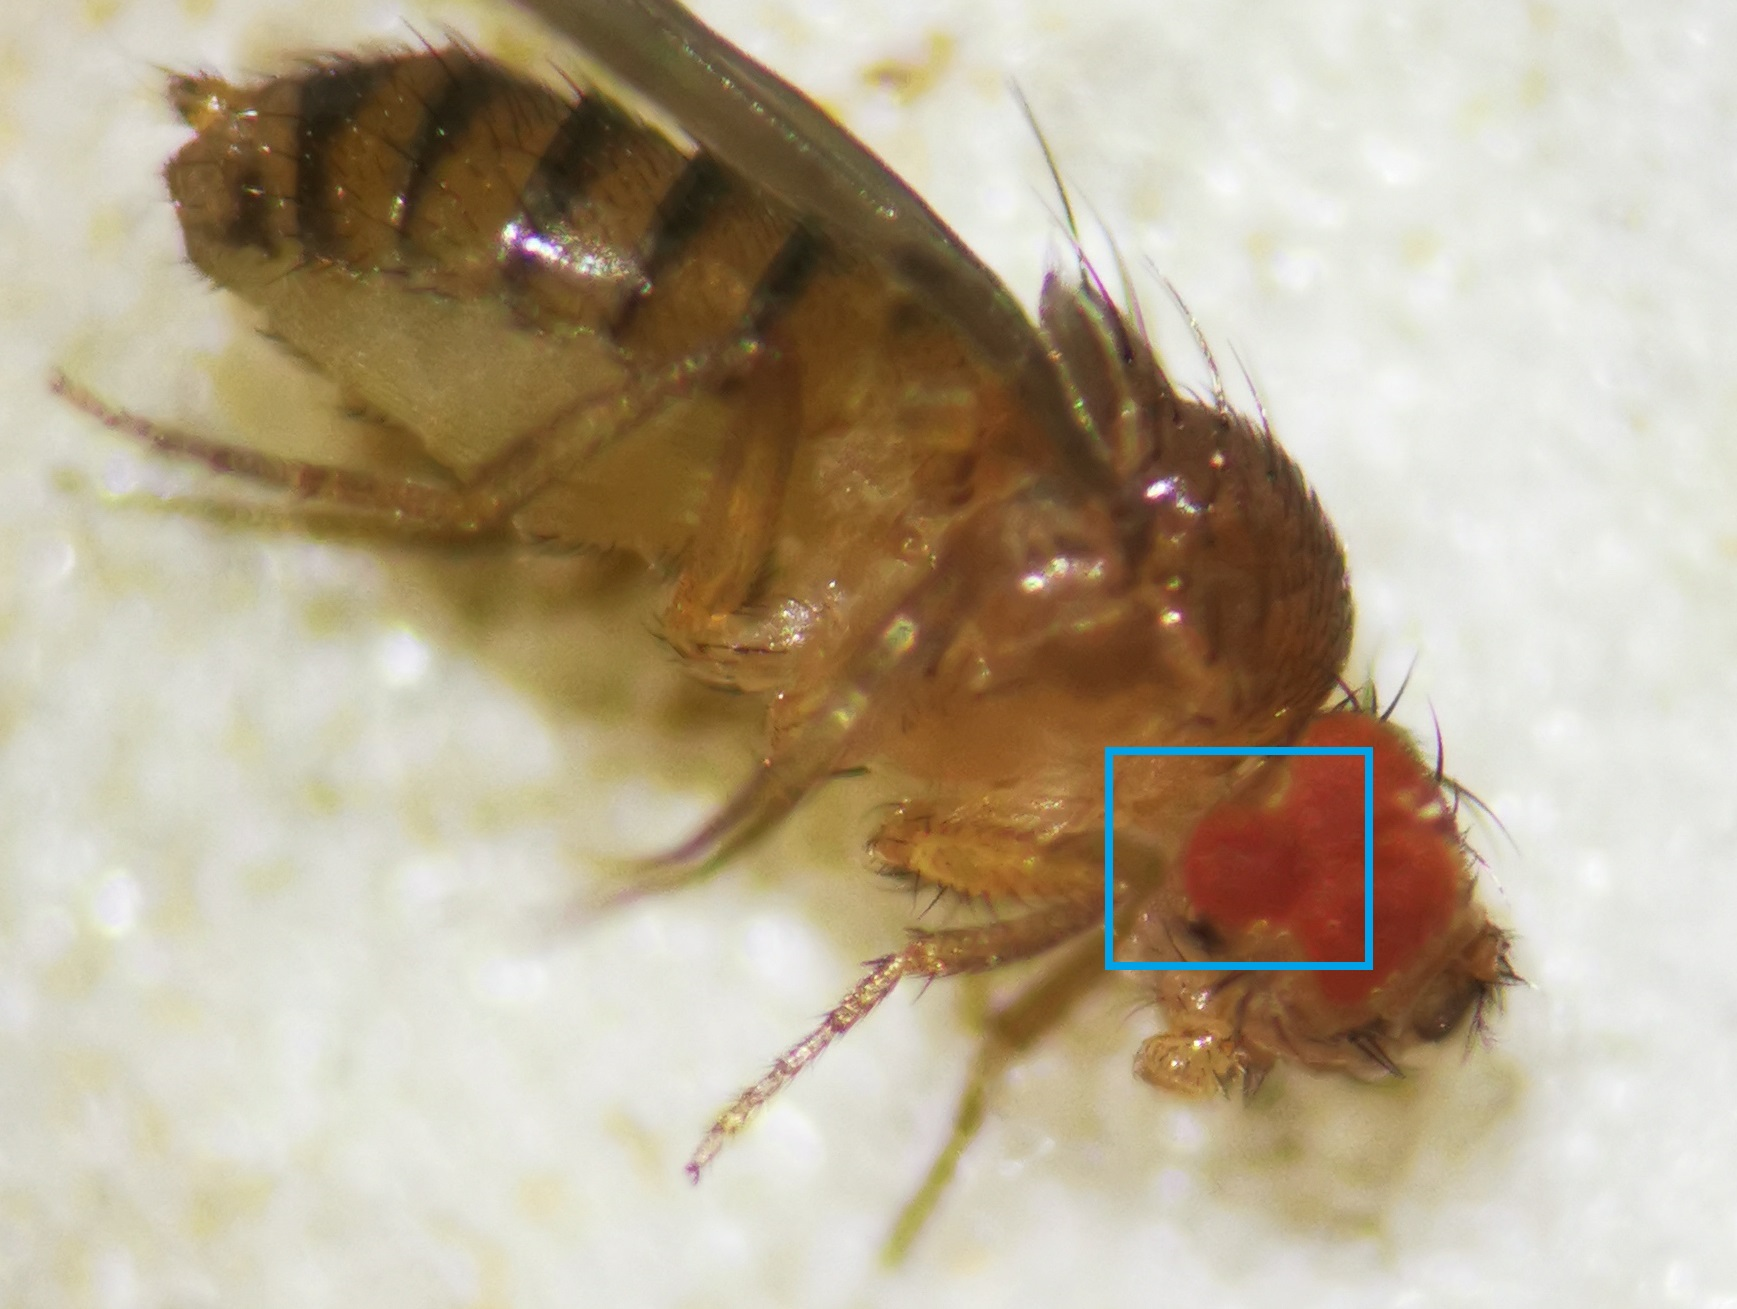
\includegraphics[width=0.5\textwidth,angle=0]{image/Eye.jpg}
    \caption{A typical result of eye tumour metastases}
    \label{Eyef}
\end{figure}

The ratio of eye tumour metastases is shown in the figure below.
\begin{figure}[H]
    \centering
    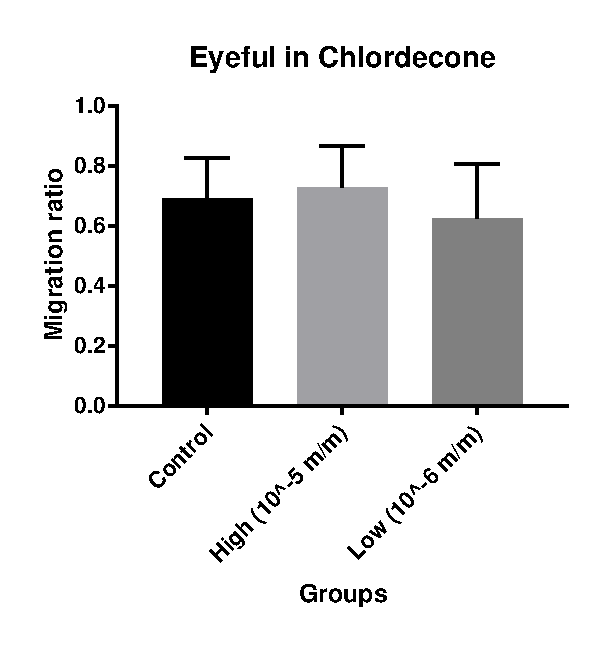
\includegraphics[width=0.6\textwidth,angle=0]{image/Data1.eps}
    \caption{The ratio of eye tumour metastases}
    \label{Eye}
\end{figure}



\subsubsection{Survival curve}
The survival curve of parent adults in different environments is shown in the figure below.
\begin{figure}[H]
    \centering
    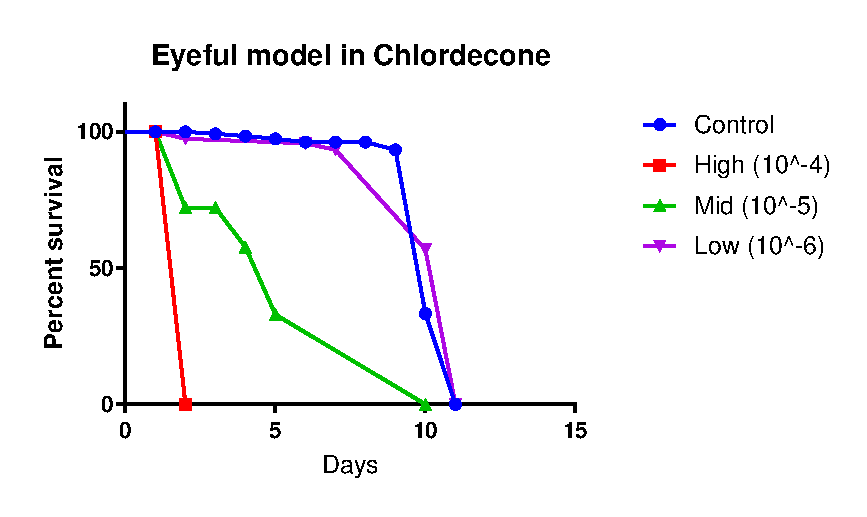
\includegraphics[width=0.7\textwidth,angle=0]{image/Data3.eps}
    \caption{Survival curve of parent adults}
    \label{D3}
\end{figure}



\subsubsection{Discussion}
Due to the small number of samples (n=12 for control group, n=11 for $10^{-5}$ group, n=8 for $10^{-6}$ group), the t-test did not give out significant results, but the figure suggests a tendency of hormesis. Low concentration seems to repress the tumour metastases, while 10 folds higher concentration leads to slightly more tumour metastases.

The fact that no significant changes can be found in tumour metastases may result from the difference in the survival rate of parent adults, which is confirmed by the survival curve and the statistical analysis (**** significance). Low F1 survival rate indicates a low survival rate of the F1, which can balance the influence of Chlordecone on tumour metastases.